\documentclass[preview,float]{standalone}
\usepackage{tikz}
\usetikzlibrary{hobby,decorations.markings}
\usepackage{graphicx}

\begin{document}
\begin{tikzpicture}
\draw[green,
  postaction={
    decorate,
    decoration={
      markings,
      mark=between positions 0 and 1 step 0.33 with
      {
        \node[transform shape] {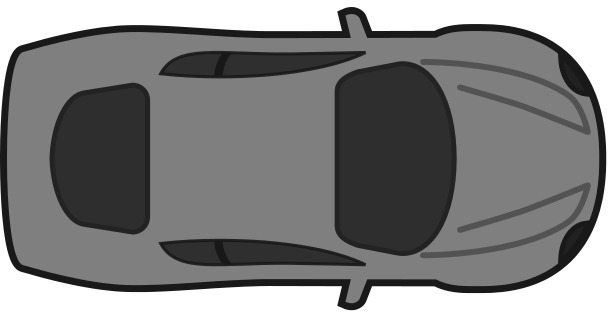
\includegraphics[width=.5cm]{car}};
      }
    }
  }
]
(0,0) to[out angle=0,in angle=180,curve through={(1,.35) .. (2,0.40) .. (3,.35)}] (4,0);

\draw[red,
postaction={
	decorate,
	decoration={
		markings,
		mark=between positions 0 and 1 step 0.5 with
		{
			\node[transform shape] {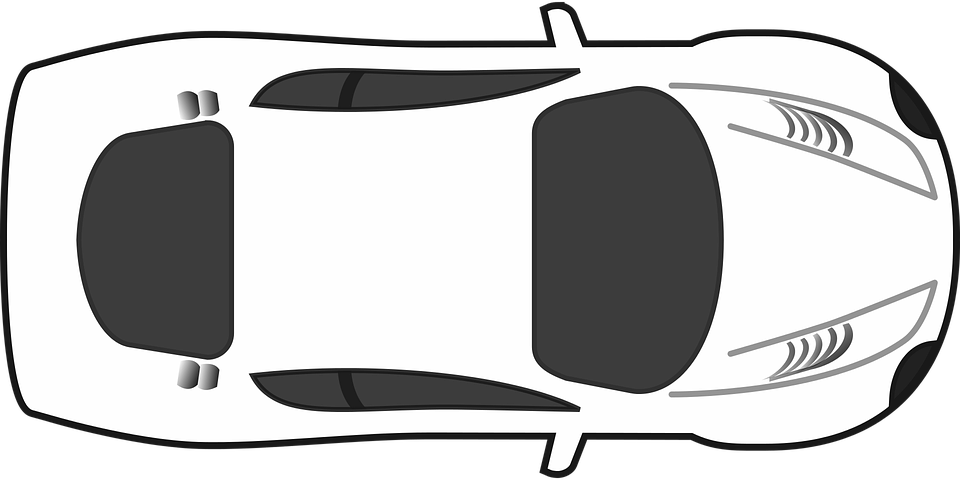
\includegraphics[width=.5cm]{obstacle}};
		}
	}
}
]
(1,0) to[out angle=0,in angle=180] (3,0);

\draw[dashed]
(-0.5,0.165) to[out angle=0,in angle=180] (4.5,0.165);
\draw
(-0.5,-0.2) to[out angle=0,in angle=180] (4.5,-0.2);
\draw
(-0.5,0.6) to[out angle=0,in angle=180] (4.5,0.6);

\end{tikzpicture}
\end{document}